\documentclass{article}
\usepackage{graphicx} % Required for inserting images
\usepackage[top=0.9in, bottom=1in, left=1.0in, right=1.0in]{geometry}
\usepackage[utf8]{inputenc}
\usepackage[icelandic]{babel}
\usepackage[T1]{fontenc}
\usepackage[sc]{mathpazo}
\usepackage[parfill]{parskip}
\renewcommand{\baselinestretch}{1.2}
\usepackage{booktabs,tabularx}
\usepackage{multirow}
\usepackage{enumerate}
\usepackage{adjustbox}
\usepackage{multicol}
\usepackage{xcolor}
\usepackage{algpseudocode}
\usepackage{tikz}
\usepackage{nicefrac}
\usepackage{changepage}
\usetikzlibrary{arrows, positioning, calc, graphs}
\usepackage{amsmath, amsfonts, amssymb, amsthm}
\usepackage{graphicx}
\usepackage{tikz}
\usepackage{minted}
\usemintedstyle{manni}
\title{Tölvutækni og Forritun Verkefni 2}
\author{Ragnar Björn Ingvarsson, rbi3}
\tikzset{->, >=stealth', shorten >=1pt, node distance=2cm,thick, main node/.style={circle,draw,minimum size=3em}}

\begin{document}
\renewcommand\thepage{}

	\maketitle

	\newpage
	\setcounter{page}{1}
	\renewcommand\thepage{\arabic{page}}
	\renewcommand\thesection{\Roman{section}}
	\renewcommand\thesubsection{\Roman{section}.\roman{subsection}}

	\section{Skrifa hermi fyrir skyndiminni}
	\begin{minted}{c}
void initCache()
{
    cache = (cache_set_t*) malloc(S*sizeof(cache_set_t));
	for (int i = 0; i < S; i++) {
		cache[i] = (cache_line_t*) malloc(E*sizeof(cache_line_t));
	}
}

void freeCache()
{
	free(cache);
}

void accessData(mem_addr_t addr)
{
	long set = (addr >> b) & ((1ULL << s) - 1);
	long tag = addr >> (s+b);

	int has_hit = 0;
	int insert_place = -1;
	int lowest_value = policy_code == 1 ? cache[set][0].lru : cache[set][0].fifo;
	int lowest_index = 0;

	for (int i = 0; i < E; i++) {

		cache_line_t line = cache[set][i];

		if (policy_code == 1) {
			if (lowest_value > line.lru) {
				lowest_value = line.lru;
				lowest_index = i;
			}
		} else if (policy_code == 2) {
			if (lowest_value > line.fifo) {
				lowest_value = line.fifo;
				lowest_index = i;
			}
		}

		if (line.valid && line.tag == tag) {
			line.lru = ++lru_counter;
			hit_count++;
			has_hit = 1;
			cache[set][i] = line;
			break;
		}
		if (!line.valid) {
			insert_place = i;
		}
	}
	if (!has_hit) {
		miss_count++;
		if (insert_place == -1) {
			insert_place = policy_code == 3 ? rand() % E : lowest_index;
			eviction_count++;
		}
		cache_line_t line_to_be_added;
		line_to_be_added.tag = tag;
		line_to_be_added.fifo = fifo_counter++;
		line_to_be_added.lru = lru_counter++;
		line_to_be_added.valid = 1;
		cache[set][insert_place] = line_to_be_added;
	}
}
	\end{minted}

	\vspace{6em}

	\begin{center}
		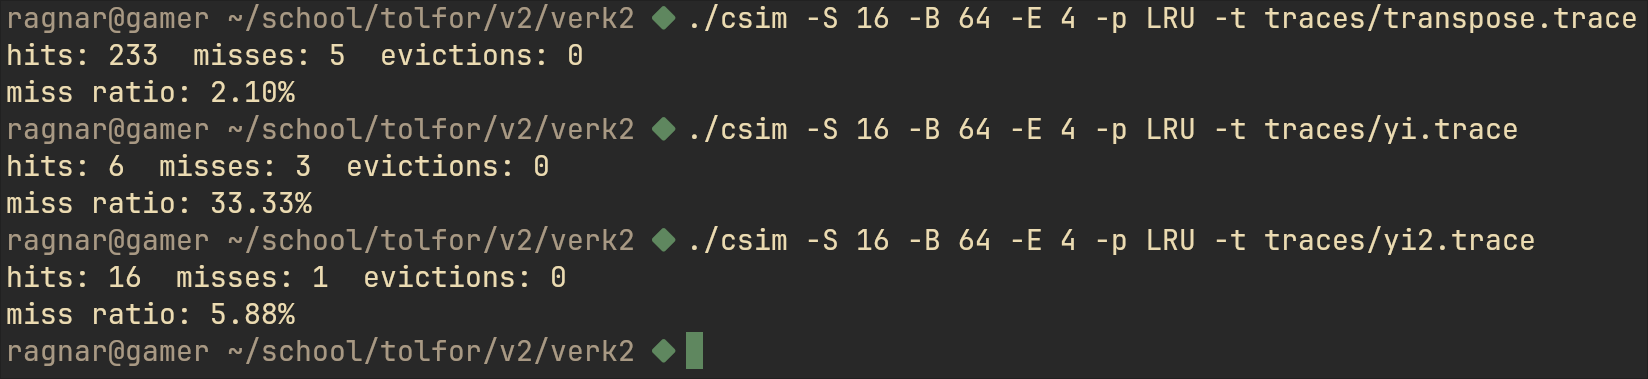
\includegraphics[width=0.95\textwidth]{result.png}
	\end{center}

	\newpage
	\section{Besta uppsetning á skyndiminni}
	\begin{multicols}{2}
	\begin{figure}[H]
		\begin{center}
			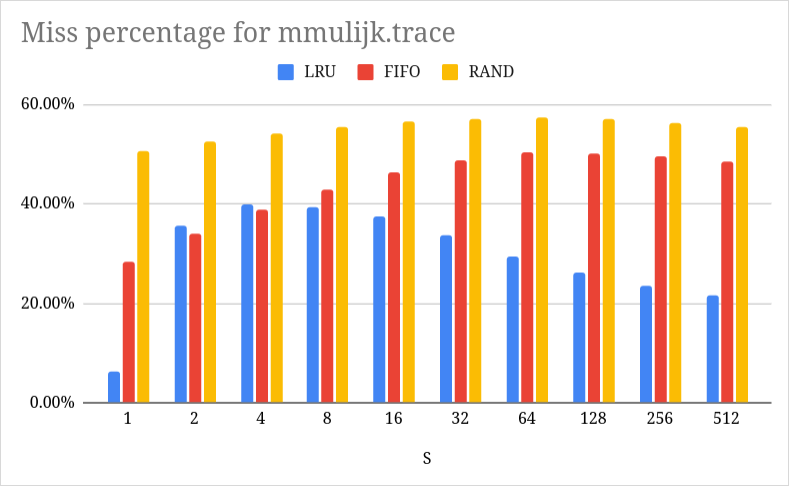
\includegraphics[width=0.48\textwidth]{mmul.png}
		\end{center}
		\caption{\texttt{mmulijk.trace}}\label{fig:mmul}
	\end{figure}
	\begin{figure}[H]
		\begin{center}
			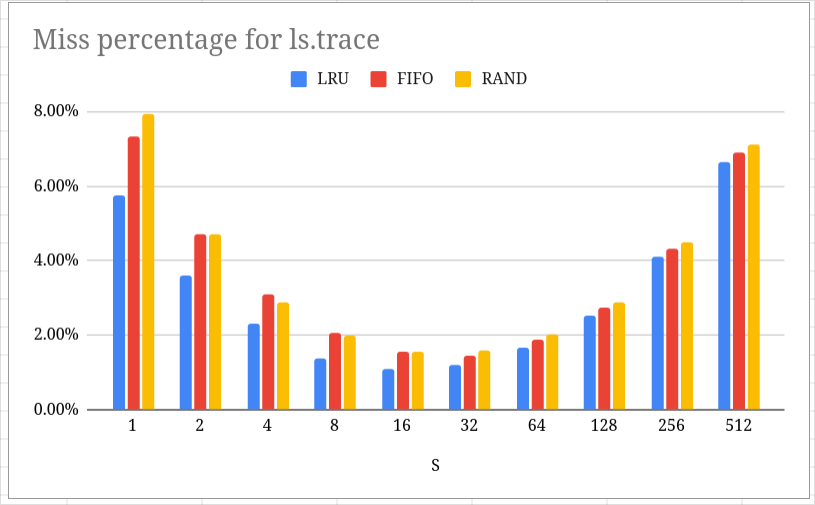
\includegraphics[width=0.48\textwidth]{ls.png}
		\end{center}
		\caption{\texttt{ls.trace}}\label{fig:ls}
	\end{figure}
	\end{multicols}
	
	\subsection{Hver er munurinn á bestu uppsetningu á milli 
	rakningaskránna?}


	\subsection{Hvernig kemur uppsetning Intel Core i7 út í hermunum?}
	
\end{document}
